\chapter{Complementos de Scrum}

Scrum no tiene como objetivo dar instrucciones precisas a los equipos sobre la forma concreta en la que deben llevar a cabo su desarrollo. Scrum espera que los equipos hagan lo que sea necesario para ellos para entregar el producto de calidad. Las prácticas y herramientas de desarrollo cambian y mejoran de manera continua y los buenos equipos trabajarán constantemente en pos de obtener el mejor uso de las mismas. Desde esta perspectiva, se puede consensuar en un anillo de complementos útiles que rodea el núcleo de Scrum y que pueden potenciar el trabajo ágil y la práctica de ingeniería. Estos complementos son métodos y técnicas complementarias a Scrum, sujerencias y recomendaciones, lecciones aprendidas y conceptos aledaños. En este capítulos trataremos estos temas.

% Malas prácticas, consejos, tecnicas complementarias, casos de estudios

%Técnicas para requerimientos
% Historias de usuarios
% Técnica Killen :  sirve para definir cuales son las cuestiones clave a desarrollar en un proyecto y su priorización logrando un conjunto de historis de usuario.
% Mapas de historia (Técnica propuesta por Jeff Patton)
% Articles: The New User Story Backlog is a Map By Jeff Patton. JPattonAssociates.com, Octuber 8, 2008.
% URL: http://jpattonassociates.com/the-new-backlog/
%Técnicas de Planeación
%Técnicas de estimación
% Poker de planeación
%Técnicas de Comunicación
% Radiadores de información
% Scrum task board
% Comunicación osmótica
% -----------técnica que te permita limitar la cantidad de trabajo en progreso y la priorización de las tareas, como % son la Técnica pomodoro y la Matriz de Eisenhower respectivamente.
%Técnicas de Programación

\newpage
\section{Técnicas para requerimientos}

\subsection{Historias de usuarios}

Para Scrum las hipótesis de requerimientos se representan en items de Backlog de producto PBI. A estos PBIs se los suele denominar "Story" o "Historias de Usuarios"\footnote{Las "User Story" son una técnica de eXtremme Programming (XP)}. El Product Backlog incluye incisos o Stories que aportan valor al cliente y que suelen ser descripción de requisitos funcionales. Aunque también puede incluir entradas para exploración de características, necesidades del cliente u opciones técnicas, requerimientos no funcionales, el trabajo necesario para lanzar el producto, y otros incisos, así como la configuración del entorno o arreglar defectos \footnote{\cite{Scrum-Institute-2015}}. O sea que puede proporcionar valor en forma indirecta mediante el aumento de la calidad o la reducción de los incidentes en el largo plazo \footnote{\cite{Scrum-Institute-2015}}.

Las historias representan un concepto verificable y simple, que el Product Owner quiere implementar en el producto. Según el concepto general de metodología Ágil, la historia se define como una "promesa de una conversación" o una "descripción de una característica" \footnote{\cite{UNTREF-2014}, \cite{Dan-North-2015}}. Según esta perspectiva, la historias de usuario representa una "funcionalidad de aplicación" para un usuario y que brinda un beneficio (ROL + FUNCIONALIDAD + BENEFICIO). Las mismas se escriben siempre con lenguaje de negocio y respetando la siguiente pauta de estructura:\newline

\textbf{COMO} <ROL> \textbf{QUIERO} <FUNCIONALIDAD> \textbf{PARA QUE} <BENEFICIO>\newline

Por ejemplo:

%Example of User Story
\begin{itemize}
\item \textbf{COMO} ScrumMaster 
\item \textbf{QUIERO} que las reuniones no se extiendan más de un tiempo consensuado 
\item \textbf{PARA QUE} no se pierda el foco.
\end{itemize}

La historia de usuario no es exactamemte un requerimiento, pero puede considerarse como el título de una hipótesis de requerimiento como recordatorio de algo relevante a conversar con el usuario o cliente. En consecuencia lo relevante es su evolución como conversación \footnote{\cite{UNTREF-2014}}.

La historia de usuario describe lo que el usuario quiere hacer desde la perspectiva de una interacción con un proceso de negocio, describe el objetivo del usuario en términos de necesidad de obtener algo que se hace en el negocio \footnote{\cite{Scott-Bellware-2008}}.

Según Dan North y en el marco de Behavior-Driven Development (BDD), una Story es más un requerimiento, pues tiene que ser una descripción de un requisito y su beneficio para el negocio, y un conjunto de criterios con los que todos estamos de acuerdo de qué es o lo que se hace, "lo que el cliente necesita" \footnote{\cite{Dan-North-2015}}. 

\subsubsection{Criterio de demarcación}

Las historias de usuario bien escritas son esenciales para el desarrollo ágil y la ingeniería de software. Existen ciertas características a tener en cuenta a la hora de escribir una historia de usuario y determinar cuál es una bien escrita o una válida. El criterio de demarcación aceptado en metodología ágil en general es el criterio INVEST\footnote{INVEST es un acrónimo creado por Bill Wake.} y que consta de seis características a cumplir \footnote{\cite{UNTREF-2014}, \cite{Scrum-Alliance-2015}}:

\begin{enumerate}

\item \textbf{Independiente:} una historia debe ser atómica. Es decir que se debe buscar asegurar la cohesión funcional y el bajo acoplamiento entre historias distintas. La fuerte dependencia entre diferentes historias hace que sea más dificil planificar, priorizar y estimar.

\item \textbf{Negociable:} debe ser conversable y en consecuencia negociable (es viva). Las historias "no son requerimientos contractuales"\footnote{"Las user stories no son obligaciones contractuales"\cite{Cohn-2004}} ni requisitos rígidos, y su detalle y precisión debe poder evolucionar en el tiempo en procesos de refinamiento y conversaciones en una ingeniería de requerimientos evolutiva.

\item \textbf{Valueble:} debe generar un valor al cliente (usuario o comprador). Una Story sin una declaración de la motivación del usuario a menudo se piensa que es no accionable; es decir, la historia no se puede estimar o implementar fácilmente \footnote{\cite{Scott-Bellware-2008}}. Lo ideal, además de la declaración explícita del beneficio, es que haya una forma de medir el valor que aporta al cliente.

\item \textbf{Estimable:} se debe poder estimar. La historia debe brindar la suficiente información que de la certidumbre necesaria para que los desarrolladores puedan estimarla y permitir, de este modo, que se pueda priorizar y planificar. 

\item \textbf{Pequeña:} debe ser lo suficientemente pequeña para entrar en un sprint o iteración. El tamaño pequeño de las historias ayuda a reducir el tamaño del lote, incrementar el flujo de valor hacia el cliente y asegurar que cada miembro del equipo de desarrollo pueda hacer una contribución valiosa cada día. Por ejemplo, en cada Sprint se podrían completar entre cuatro y ocho historias pequeñas. A medida que una historia es más grande va a tener más errores asociados a la estimación y alcance, y aumentará la probabilidad de terminar en un Sprint fallido.

\item \textbf{Probable:} debe poder permitir la contrastabilidad. La contrastabilidad del enunciado de la historia es la propiedad de ésta de ser capaz de ser sometida a una prueba empírica y repetible a fin de evaluar su adecuación o no a los hechos a los que se refiere o resultados esperados. Esta característica es crucial para hacer ingeniería, sin la contrastabilidad no se hace ingeniería. Un ejemplo de historia no probable sería: "Como usuario quiero un software hermoso y facil de usar".

\end{enumerate}

\subsubsection{¿Qué NO es una Historia de Usuario?}

Si no cumple con el criterio INVEST es bastante probable que no sea una Story. Por ejemplo una tarea puramente técnica (que le interesa solo al desarrollador), un refactoring técnico o un Spike no cumplen con INVEST y en su generalidad no son Story. 
Veamos los siguientes ejemplos:

\begin{itemize}

\item \textbf{Spike:}
No es una Story ya que es una tarea de investigación y/o experimentación en formato time-boxing por lo que no cumple con ser probable ni estimable (no cumple con dos criterios).

\item \textbf{Refactoring Task:}
Es una tarea técnica de reingeniería que no es valuable o su valoración es a futuro o en relación a un atributo de calidad que puede no estar directamente solicitado por el cliente o no impacta en beneficio inmediato para el cliente, ya que podría estar resolviendo una "deuda técnica"\footnote{Deuda técnica es la incurrida involuntariamente debido a trabajos de baja calidad o deuda incurrida intencionalmente (McConnell, Ward Cunningham) y que consta en arquitectura no escalable, defectos en el código, documentación inservible o desactualizada, problemas para migrar o actualizar funcionalidades o problemas por falta de mantenimiento.}. Esto no quiere decir que no pueda haber una "story de refactoring" que puede proporcionar valor en forma indirecta mediante el "aumento de la calidad o la reducción de los incidentes en el largo plazo".

\item \textbf{Technical Story:}
“Cada historia tiene que ser valorada por los usuarios. Pero eso sería un error."\footnote{\cite{Cohn-2004}} Pues en realidad, una historia de usuario describe la funcionalidad que será valiosa para un usuario o comprador de un sistema o software \footnote{\cite{Cohn-2004}}. Hay historias que especifican aspectos técnicos que no son valiosos para el usuario sino mas bien para el cliente o comprador (la valoración es transitiva y no directa). Historias técnicas pueden ser valorados por los compradores que contemplan la compra del producto, pero no serían valorados por los usuarios reales. Pero esto no es lo que podemos llamar una "Technical Story" sino que es una Story con aspectos técnicos que tiene valor para el cliente. Para Scott Ambler en Agile Modeling, una Story es una definición de muy alto nivel de un requerimiento que puede ser funcional o no, por ejemplo de un requerimiento técnico \footnote{\cite{Scott-Ambler-2015}}, por ejemplo: "como usuario quiero que las transcripciones estén disponibles en línea a través de un navegador estándar lo que me permite acceder desde cualquier lugar"\footnote{\cite{Scott-Ambler-2015}}.

Cuando se habla de "Technical Story" se referencia a aquella historia técnica que sólo es valorada por los desarrolladores. Estas historias son las que se quieren evitar y considerar como Technical Story que podría ser una tarea técnica o una historia mejor redactada. Este tipo de historias se centran en la tecnología y las ventajas para los programadores. Es muy posible que las ideas detrás de estas historias sean buenas, pero en cambio deben ser escritas para que los beneficios a los clientes o usuarios sean evidentes. Esto permitirá que el cliente priorizar inteligentemente estas historias en el calendario de desarrollo \footnote{\cite{Cohn-2004}}.

Para la Agile Alliance una Story no se corresponde en general a un "componente técnico" o de la "interfaz de usuario", pues a pesar de que a veces puede ser un atajo útil hablar de por ejemplo "la historia de diálogo de búsqueda", pantallas, cuadros de diálogo y botones, no son historias de usuario \footnote{\cite{Scrum-Alliance-2015}}.

\end{itemize}

\subsubsection{Componentes de una Historia de Usuario}

Las historias de usuarios se componen de tres elementos comunmente denominados las tres 'C'\footnote{Las 3 Cs de Ron Jeffries.}:

\begin{enumerate}

\item \textbf{Carta o tarjeta (Card):} Las historias se deben poder escribir en una tarjeta de papel pequeña. Por ese motivo la redacción de las mismas debe ser clara, precisa y concisa para caber en una tarjeta de papel.

\item \textbf{Conversación:} Las historias deben tener y generar conversaciones cara a cara entre el Product Owner y el Equipo de Desarrollo.

\item \textbf{Confirmación:} Deben estar suficientemente explicada para que el Equipo de Desarrollo qué es lo que se desea construir y qué es lo que se espera como resultado de dicha implementación. La confirmación es el "Criterio de Aceptación" que los desarrolladores deben tener en cuenta para que la misma sea aceptada por el cliente.

\end{enumerate}

\subsubsection{Criterio de Aceptación}

Las historias de usuario tienen límites específicos para las características del producto, proceso o servicio definido en la hipótesis de requerimiento que determinan los resultados esperados para que la historia sea aceptada por el cliente. En otras palabras, el criterio de aceptación es el conjunto de afirmaciones útiles para que el cliente valide la historia.

La estructura de un criterio de aceptación presentado como escenario puede ser como la siguiente:

%Criterio de aceptación ejemplo con un escenario
\begin{itemize}
\item \textbf{Scenario 1:} Título
  \begin{itemize}
  \item \textbf{Given} [contexto] And [otro contexto]...
  \item \textbf{When}  [evento] 
  \item \textbf{Then}  [resultado] And [otro resultado]...
  \end{itemize}
\end{itemize}
  
\newpage
\section{Técnicas de Estimación}

\subsection{Puntos de historia}

Los puntos de historia o "Story Points" son una medida relativa de estimación de una historia de usuario para poder medir su tamaño y útil para medir la velocidad de un equipo. Se usa para hacer estimaciones relativas, que quiere decir que las historias se comparan entre si, buscando mantener una relación proporcional entre ellas según sus puntos de historia. O sea que si se piensa a nivel de esfuerzo, una historia que tiene 3 puntos de historia requerirá tres veces más de esfuerzo que una que sea de un punto historia.

Hay que tener en cuenta que "bajo ningún punto de vista la estimación (en story points) es un compromiso"\footnote{\cite{UNTREF-2014}} y que los puntos de historia no son medidas objetivas convertibles en forma precisa a horas. Justamente se usan puntos de historia para no estimar en horas hombre.

\subsection{Poker de planeación}

El Poker de planeación o "Planning Poker"\footnote{El "Planning Poker" proviene de un paper presentado por James Greening llamado "cómo evitar análisis parálisis en la planificación de liberaciones"\cite{James-Grenning-2002} donde se basa en el método Wideband Delphi para realizar la estimación de requerimientos de forma colaborativa. Luego el método fue popularizado por Mike Cohn con su libro "Agile Estimating and Planning"\cite{Cohn-2005}} es una técnica de estimación y planificación ágil que se basa el consenso por sabiduría de grupo. 

La dinámica consiste en que el Product Owner inicia leyendo una historia de usuario ágil o describe una característica para los desarrolladores estimadores. Cada estimador posee una baraja de "Cartas de Poker de Planificación". Los valores representan el número de puntos de la historia, día ideal, u otras unidades en las que el equipo estima. Los estimadores discutir la función, haciendo preguntas al Product Owner, según sea necesario. Cuando la función se ha discutido plenamente, cada estimador selecciona de forma privada una tarjeta a representar a su estimación. Todas las tarjetas se revelaron a continuación, al mismo tiempo. Si todos los estimadores seleccionan el mismo valor, que se convierte en la estimación. Si no, los estimadores discuten sus estimaciones. Los estimadores de valores altos y bajos deben compartir sus razones. Tras un nuevo debate, cada estimador vuelve a seleccionar una tarjeta de estimación, y todas las tarjetas se revelan de nuevo al mismo tiempo. El proceso se repite hasta que se logre el consenso, o hasta que los estimadores deciden que la estimación ágil y planificación de un ítem en particular debe ser diferida hasta que la información adicional se puede adquirir.


\subsubsection{Cartas de Poker de Planificación}

Las Cartas de Poker de Planificación que más se usan son las de Fibonacci y las de talles de remeras:

\begin{enumerate}

\item \textbf{Talles de remeras:} Las cartas de talles contempla los valores XS (muy pequeño), S (Pequeño), M (Mediano), L (grande), XL (muy grande) y XXL (extra grande). Estos valores sirven para estimar épicas, tamaños de historias o trabajo a alto nivel. 

\item \textbf{Fibonacci:} Las cartas Fibonacci contempla los valores 0, 1, 2, 3, 5, 8, 13, 20, 40 y 100, que es la secuencia fibonacci que se suele recomendar. Estos valores son útiles para estimar complejidad de historias o trabajo a nivel medio. Realizando una estimación relativa, estos valores corresponden a puntos de historia.

\end{enumerate}

\newpage
\section{Técnicas de Comunicación}

\subsection{Hacer silencio}

Una técnica para lograr silencio en un grupo es pedir silencio cuando se levanta la mano, los que ven la mano levantada tienen que callarse y levantar a su vez la mano. Cuando cualquiera ve a alguien con la mano levantada se debe callar y a su vez levantar la mano. Este comportamiento se termina propagando rápidamente en todos los integrantes hasta que se logra el silencio. Es una técnica muy útil en la reuniones cuando las personas se dispersan comunicándose en forma caótica o cuando alguna actividad de conversación libre se extiende del tiempo necesario.


\subsection{Gestión visual}

La gestión visual es la utilización de elementos y técnicas visuales, como complemento de Scrum, para la organización del trabajo y la irradiación visual del trabajo. Es aconsejable que los irradiadores de información presenten las siguientes características:

\begin{enumerate}

\item \textbf{Ubicación ostensible:} estar ubicado en el lugar de trabajo en forma de afiches, carteles o pizarras visibles.

\item \textbf{Soporte físico:} estar hechos de material tangible como papel en vez de usar software, salvo el caso de monitores grandes.

\item \textbf{Resumen autoexplicativo:} contener información importante autoexplicativa y didáctica.

\end{enumerate}

Ejemplos de irradiadores de información son: el gráfico burndown, indicadores de estados del build (usando semáforos), métricas de errores, riesgos activos, impedimentos. etcétera.

\subsection{Tableros Scrum/Kanban}

El tablero Scrum/Kanban o "Scrum Kanban Board" es una técnica que consiste en utilizar un tablero Kanban (ver figura \ref{fig:ScrumKanbanBoard}), como irradiador de información, para el manejo del cilo de estados de las tareas y de los impedimentos. El tablero Kanban debe ser visible por todo el equipo y por lo tanto transparente para todos los involucrados. Por ejemplo, durante una Daily Scrum todo el equipo es capaz de ver qué tareas se resuelven, cuáles no se han abordado todavía y qué impedimentos existen.

\subsubsection{Ejemplo de un Scrum kanban board}

Ver figura \ref{fig:ScrumKanbanBoard}.

\begin{figure}[h]
  \centering
  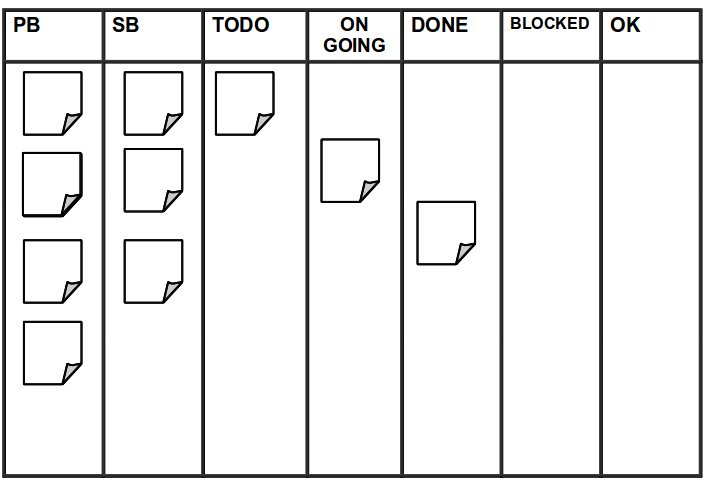
\includegraphics[width=0.9\textwidth]{ScrumKanbanBoard}
  \caption{Tablero Kanban para Scrum}
  \centering
  \label{fig:ScrumKanbanBoard} %\ref{fig:ScrumKanbanBoard}
\end{figure}

\subsubsection{Ejemplo de un Scrum board}

Un Scrum board, Kamban Board o taskboard físico (Ver figura \ref{fig:ScrumBoard}) es una tabla donde se colocan postick representando tareas.

\begin{figure}[h]
  \centering
  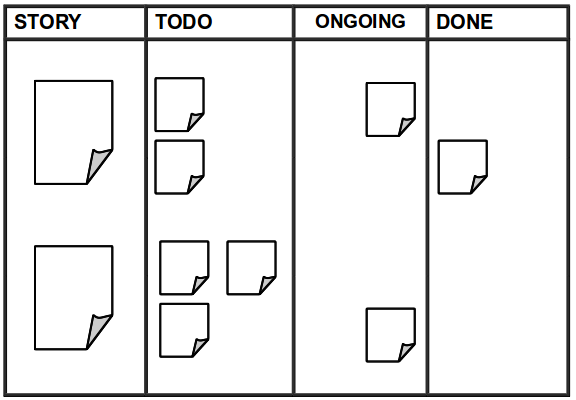
\includegraphics[width=0.8\textwidth]{ScrumBoard}
  \caption{Tablero Scrum}
  \centering
  \label{fig:ScrumBoard} %\ref{fig:ScrumBoard}
\end{figure}

\subsection{Tablero de Obstáculos}

El Tablero de Obstáculos (ver figura \ref{fig:ObstacleBoard}) es una herramienta visual útil para hacer seguimiento de los obstáculos o bloqueos del equipo que surgen en el trabajo del Sprint. El dueño del Tablero de Obstáculos es el Scrum Master, quien se encarga de buscar remover todos los obstáculos que puedan paralizar o ralentizar el trabajo del equipo o desviarlo de su foco esencial. El tablero tanbién le es útil al equipo para tener la visibilidad del estado de los obstáculos.

Ver figura \ref{fig:ObstacleBoard}.

\begin{figure}[h]
  \centering
  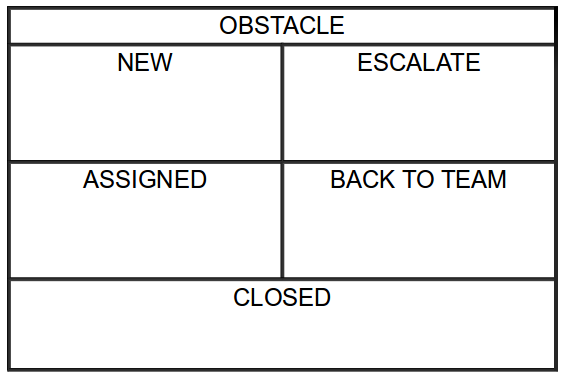
\includegraphics[width=0.6\textwidth]{ObstacleBoard}
  \caption{Tablero de Obstáculos}
  \centering
  \label{fig:ObstacleBoard} %\ref{fig:ObstacleBoard}
\end{figure}

\subsection{Gráficos de esfuerzo pendiente}

\subsubsection{Gráfico Burndown}

Un gráfico de trabajo pendiente o "Burndown charts"\footnote{El Burndown muestra la cantidad de trabajo que queda. \cite{SBOK-2013}} (figura \ref{fig:Burndown_chart}) es uno que muestra el trabajo restante o que queda por hacer versus tiempo. Muestra la velocidad a la que se están completando los PBIs o historias reflejando el avance y permitiendo extrapolar si el Equipo podrá completar el trabajo en el tiempo restante.

\begin{figure}[h]
  \centering
  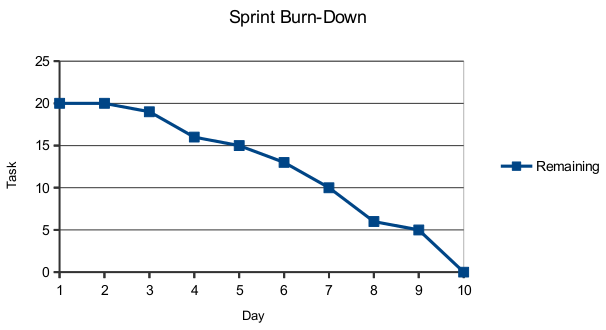
\includegraphics[width=0.9\textwidth]{Burndown_chart}
  \caption{Gráfico Burndown}
  \centering
  \label{fig:Burndown_chart} %\ref{fig:Burndown_chart}
\end{figure}

Se pueden utilizan dos gráficos de esfuerzo pendiente:

\begin{enumerate}

\item \textbf{Burndown de Sprint:} Días u horas pendientes para completar las tareas de la iteración (sprint burndown chart), realizado a partir de la lista de tareas de la iteración. Normalmente se utiliza para saber cuánto falta para terminar las historias comprometidas en un Sprint. Es un diagrama de dos ejes: en el eje X el tiempo en días de duración del sprint, en el eje Y la cantidad de trabajo comprometida con el cliente durante el sprint en las unidades que se hayan acordado.

\item \textbf{Burndown de Proyecto:} Días pendientes para completar los requisitos del producto o proyecto (product burndown chart), realizado a partir de la lista de requisitos priorizada (Product Backlog).

\end{enumerate}

\subsubsection{Gráfico Burn-Up}

El gráfico de trabajo realizado o Burn-up\footnote{El Burnup muestra el trabajo realizado como parte de la Sprint. \cite{SBOK-2013}} (figura \ref{fig:Burnup_chart}) es muy similar al Burndown, con la diferencia de que se parte del cero, y se va marcando la cantidad de trabajo completado en el Sprint. En este gráfico la curva va hacia arriba asercándose a una línea que representa el alcance comprometido. En este tipo de gráfico es más fácil visualizar los cambios de alcance.

\begin{figure}[h]
  \centering
  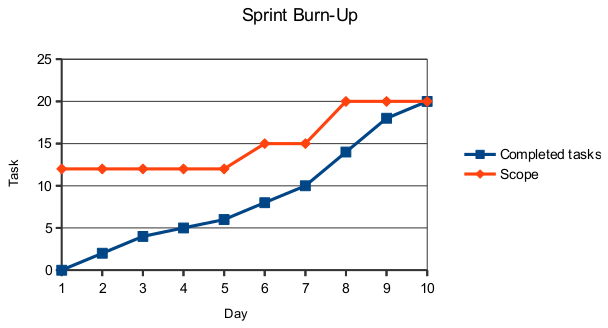
\includegraphics[width=0.9\textwidth]{Burnup_chart}
  \caption{Gráfico Burnup}
  \centering
  \label{fig:Burnup_chart} %\ref{fig:Burnup_chart}
\end{figure}

\newpage
\section{Técnicas de Programación}

Hay diferentes técnicas que pueden ser utilizadas en el proceso de desarrollo de software bajo el marco de Scrum. A continuación se describen algunas principales que sirven de soporte a metodologías ágiles:

\subsection{Técnica Pomodoro}

Se usa 'Pomodoro'\footnote{La Técnica Pomodoro es un método para la administración del tiempo desarrollado por Francesco Cirillo a fines de los años 1980\cite{Cirillo-Francesco-1980}.} como una técnica de gestión del tiempo y se basa en la hipótesis de que las pausas frecuentes en el trabajo pueden mejorar la agilidad mental. Por este motivo, la técnica consiste en dividir el tiempo dedicado a un trabajo en intervalos (time-boxing) de 25 minutos (llamados 'pomodoros') separados por descansos. Los primero tres descansos son de 5 minutos y el descanso despues del cuarto pomodoro es de 15 minutos, para luego repetir la secuencia en forma cíclica. Durante el intervalo pomodoro el trabajo debe ser focalizado, por lo que no se deben admitir distracciones o trabajos ajenos al trabajo principal. 
Esta es una técnica útil en el desarrollo ágil y en la programación en pareja (pair programming) además de otros contextos de trabajo.

\subsection{Programación de a pares}

La programación de a pares, “pairing” o “pair programming” consiste en que dos programadores participen conjuntamente en un esfuerzo combinado de desarrollo en un puesto de trabajo. La misma se puede extender al desarrollo de a pares (análisis, diseño, codificación, pruebas, diseño de interfaces de usuario, diseño gráfico, etc.).

Existen muchas razones por los que esta técnica es recomendable y las principales pueden ser las siguientes:

\begin{enumerate}

\item \textbf{Calidad:} Mejorar la calidad logrando reducir defectos por "revisión de a pares" mientras se programa.

\item \textbf{Aprendizaje:} Lograr el aprendizaje en equipo distribuyendo y nivelando el conocimiento. Pues, focalizarse en el aprendizaje es crucial para organizaciones scrum de equipos por características, donde todos deben manejar un conocimiento amplio y multidisciplinario. 

\item \textbf{Propiedad colectiva:}
Mejorar los diseños y las estimaciones debido a que todos tienen un conocimiento de la estructura del producto, un empoderamiento del mismo (propiedad colectiva del código) y de cómo puede impactar un cambio en parte de él.

\item \textbf{Resolución de problemas:} Permitir superar problemas difíciles de forma más simple, más rápido o al menos efectiva cuando trabajan juntos. La idea es que dos personas piensen mejor que una en resolver un problema.

\end{enumerate}

\subsection{Revisión de a pares}

La revisión de a pares o "peer review" es una práctica intrínseca de la actividad científica en un sistema de evaluación del trabajo científico, donde los miembros de la comunidad revisan los trabajos de sus pares\footnote{Formalmente el proceso de revisión por pares del trabajo científico fue iniciado en 1753 por la “Royal Society of London”.}. Por este motivo, implementar este tipo de prácticas en el desarrollo de software hace que sea una actividad ingenieril. El beneficio es lograr una mejor calidad y una reducción de defectos. Según Boehm "el 60 por ciento de los defectos de código se pueden eliminar durante las revisiones de a pares"\footnote{\cite{Boehm-2001}}. Así como en ciancia se revisan los trabajos de investigación antes de ser publicados, en ingeniería de software se revisa el código antes de ser desplegado.\newline
La práctica consiste en que una vez que el programador desarrolló un trabajo de codificación, solicite ante un colega compañero o un conjunto de ellos la inspección del código. Si se encuentran errores u observaciones, el desarrollador deberá mejorarlo y hasta que no tenga el visto afirmativo el código, no será desplegado o integrado al producto. Hay que tener en cuenta que para que la revisión por pares sea realmente productiva, debe ser ejecutada con el máximo de rigor, aunque implique retrasar despliegues de producto y no cumplir con los plazos comprometidos por el equipo. Cuando se aplica Scrum, el máximo de rigos incluye, además de la calidad del trabajo, prestar particular importancia al cumplimiento de la definición de terminado (DoD).

\subsection{Test Driven Development}

El "Test Driven Development" (TDD) o "desarrollo guiado por pruebas"\footnote{\cite{Jurado-2010}} es una práctica, técnica de desarrollo ágil y técnica de programación que hace foco en el comportamiento especificado de unidades de software\footnote{[Wikipedia 2014]} como disparador para el desarrollo de pruebas. Osea, basándose en especificaciones, esta práctica tiene como táctica escribir primero las pruebas (código de prueba) y después el código (código de producto) para luego realizar ciclos de "refactorización" \cite{Kent-Beck-2003}. Con este enfoque se pretende, entre otras cosas, que el diseño sea el código mismo (código de producto) y que las pruebas concretas (código de prueba) sirvan de documentación. Esta técnica se complementa con la automatización de pruebas. En todo ese conjunto de pruebas concretas, las pruebas de unidad se usan para validar métodos individuales y conjuntos de métodos. En consecuencia, en este tipo de desarrollos, se logran sistemas con un gran conjunto de pruebas (muchas líneas de código en pruebas).\newline
Si tenemos que asignar un lema a este enfoque es "la prueba en primer lugar" y su afirmación filosófica principal sería que "el diseño emerge del refactoring originado por pruebas".

\subsection{Integración contínua}

La integración continua (Continuous Integration\footnote{Continuous Integration fue propuesto inicialmente por Martin Fowler.}) es un modelo informático que consiste en hacer integraciones automáticas de un proyecto, compilación y ejecución de pruebas, lo más a menudo posible para así poder detectar fallos cuanto antes.
